% ------------------------------------------------------------------------------
%
% PREAMBLE
%
% ------------------------------------------------------------------------------

\documentclass[12pt, titlepage]{article}


\usepackage{graphicx, amsmath, amssymb, natbib, setspace, sectsty, verbatim, 
		mathrsfs}
\usepackage{MnSymbol}
\usepackage{multirow}
\usepackage{bm}
\usepackage[usenames, dvipsnames]{color}
\bibpunct{(}{)}{;}{a}{}{,}
\setlength{\parindent}{3em}
%\parskip = 1.5ex
%\linespread{1.3}
%\onehalfspacing

\pdfpagewidth 8.5in
\pdfpageheight 11in
\setlength{\oddsidemargin}{0.0in} \setlength{\textwidth}{6.5in}
\setlength{\topmargin}{0.15in} \setlength{\textheight}{8.5in}
\setlength{\headheight}{0.0in} \setlength{\headsep}{0.0in}

\usepackage{/mnt/ExtraDrive1/Work/shTex/mymacros}

\providecommand{\norm}[1]{\lVert#1\rVert}
\newcommand{\csection}[1]{\section[#1]{\centering #1 }}
\subsectionfont{\small}
\newcommand{\cye}[1]{\color{yellow!70!black}#1}
\newcommand{\cre}[1]{\color{red!70!black}#1}
\newcommand{\cbl}[1]{\color{blue!70!black}#1}
\newcommand{\cgr}[1]{\color{green!70!black}#1}


% ------------------------------------------------------------------------------
%
% BEGIN DOCUMENT
%
% ------------------------------------------------------------------------------

\begin{document}

\setcounter{equation}{0}
\renewcommand{\theequation}{R.\arabic{equation}}


% ------------------------------------------------------------------------------
%
%                    Section 8.6.3
%                    Comparing MLE to REMLE
%
% ------------------------------------------------------------------------------

{\large \textbf{8.6.3 The wet sulfate desposition data}}

\vspace{.3cm}

Exploratory data analysis scattered throughout Chapter 3 suggested that it would be wise to transform the wet sulfate deposition data to the square-root scale and to set aside three outliers, yielding a modified dataset that was called the clean wet sulfate deposition data.  Polynomials of orders zero through five were fitted to these modified data by OLS in Section 4.5.3, and summary statistics from these fits suggested that polynomials up to third-order (and possibly higher) were worthy of further consideration.  The analyses presented in Section 4.5.3 also suggested that spatial autocorrelation exists and is isotropic in the residuals from the quadratic fit, but perhaps does not exist in the residuals from the cubic and higher-order fits.

Here, we fit polynomial models to the clean wet sulfate deposition data once again, but this time using likelihood-based methods.  Models having polynomial mean structures up to (and including) order five and having several geostatistical covariance functions were estimated by ML and REML.  Custom R code was written showing how to using the \texttt{optim} function to minimize two times the negative loglikelihood to obtain ML and REML estimates.  The function \texttt{optim} contains multiple minimization algorithms, and we used Nelder-Mead, as mentioned earlier.  This also returns the minimized loglikelihood value, which can be used to compute AIC and other diagnostics.  For example, Figure~\ref{Fig:SO4_AIC} shows AIC computed for all polynomial models on the two spatial coordinates from the constant mean model up to a fifth-order polynomial for both independent error models and spatially-autocorrelated error model, where the spatial autocorrelation is an exponential model.
\begin{figure}[h]
  \begin{center}
	    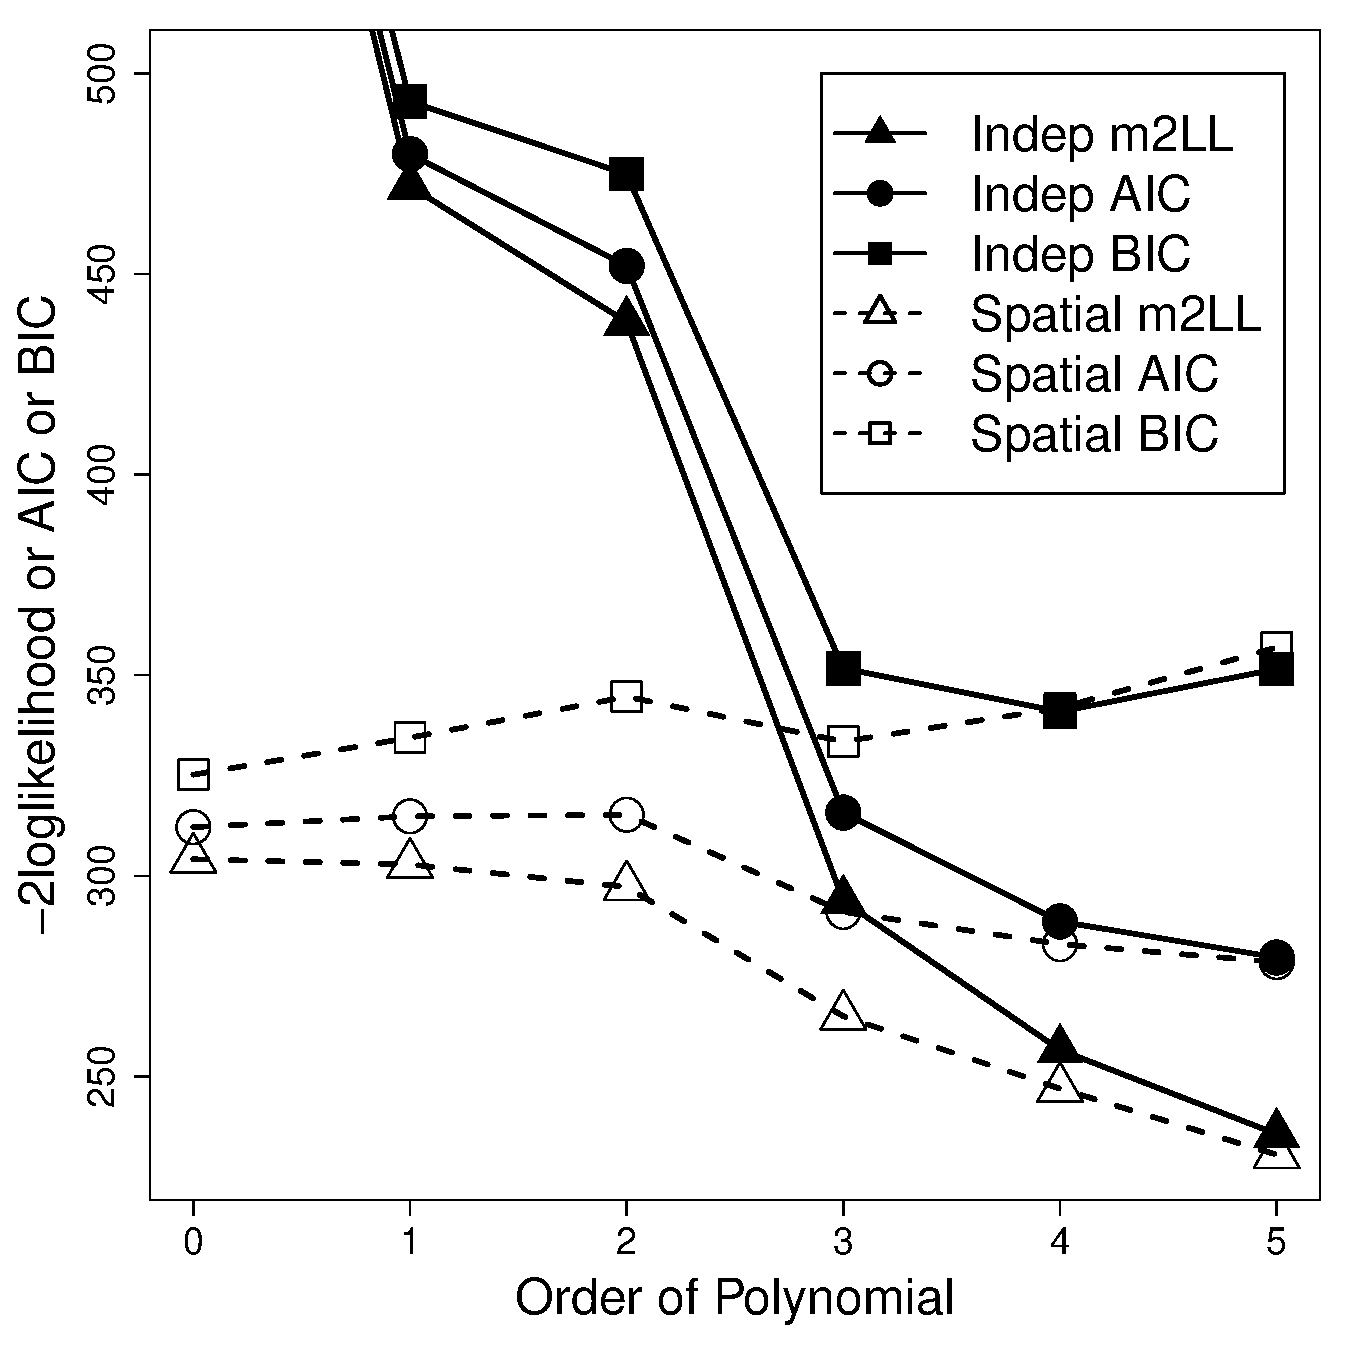
\includegraphics[width=.5\linewidth]{SO4_AIC}
  \end{center}
  \caption{AIC for polynomial models on the spatial coordinates, for both independent error models (solid line and circle) and spatial models (dashed line and open circles). \label{Fig:SO4_AIC}}
\end{figure}
Note that AIC generally decreases with the higher polynomial orders for the independent error models, while for the spatial models AIC decreases slightly to the 4th order polynomial, and starts to increase again with the fifth order polynomial.  We should point out here that AIC should be based on a likelihood minimized using ML rather than REML estimation if the column space of the fixed-effects design matrix changes among models.  REML estimation can be used in AIC to compare spatial models for a fixed-effects design matrix that does not change among models, for example, when comparing spatial autocorrelation models for an unchanging set of covariates.  AIC has a reputation for favoring overly complex models, so we also use leave-one-out cross-validation (LOOCV) and n-old cross-validation.

LOOCV eliminates one datum at a time, using all of the rest of the data to predict the one that was removed.  There is a fast and a slow way to do this.  The slow way is to remove a datum and then re-estimate all of the parameters using ML or REML estimation each time.  However, with the removal of but a single datum, the parameter estimates change very little.  A fast way to achieve LOOCV is based on holding all parameters at their values as estimated by using all of the data, and then using results from partitioned matrices so that we only have to invert the covariance matrix once (which can be saved from the ML or REML estimation, so there is in fact no additional inverses required.  Note that if a matrix is partitioned as,
$$
    \bSigma = 
    \begin{bmatrix}
       {\bSigma}_{11} & {\bSigma}_{12} \\
       {\bSigma}_{21} & {\bSigma}_{22}
    \end{bmatrix},
$$
then 
$$
    \bSigma\upi = 
    \begin{bmatrix}
       \bSigma_{11}\upi + \bSigma_{11}\upi\bSigma_{12}\bS\upi\bSigma_{21}\bSigma_{11}\upi & -\bSigma_{11}\upi\bSigma_{12}\bS\upi \\
       -\bS\upi\bSigma_{21}\bSigma_{11}\upi & \bS\upi
    \end{bmatrix},
$$
where $\bS= \bSigma_{11} - \bSigma_{12}\bSigma_{22}\upi\bSigma_{21}$ is known as the Schur complement of block $\bSigma_{22}$ of matrix $\bSigma$.  Now write $\bSigma \upi$ in block form as
$$
    \bSigma \upi = 
    \begin{bmatrix}
        \tilde{\bSigma}_{11} & \tilde{\bSigma}_{12} \\
        \tilde{\bSigma}_{21} & \tilde{\bSigma}_{22}
    \end{bmatrix},
$$
where the dimensions of the blocks in $\bSigma \upi$ follow those from the dimensions of $\bSigma$. Note that the inverse of $\bSigma_{11}\upi$ can be obtained from $\bSigma \upi$ by
$$
    \bSigma_{11} \upi = \tilde{\bSigma}_{11} - \tilde{\bSigma}_{12} \tilde{\bSigma}_{22} \upi \tilde{\bSigma}_{21}.
$$
Moreover, let us order the data such that the datum to be removed is last, so that $\bS$ is a scalar, then the inverse of $\bS$ is trivial and $\bSigma_{11} \upi$ can be computed rapidly. The main computational expense of kriging predictions rely on the inverse covariance matrix for the observed data, but in LOOCV that is given by $\bSigma_{11} \upi$, which is computed rapidly if we already have $\bSigma \upi$. 

LOOCV results for the clean wet sulfate deposition data are presented in Figure~\ref{Fig:SO4_LOOCV}.
\begin{figure}[h]
  \begin{center}
	    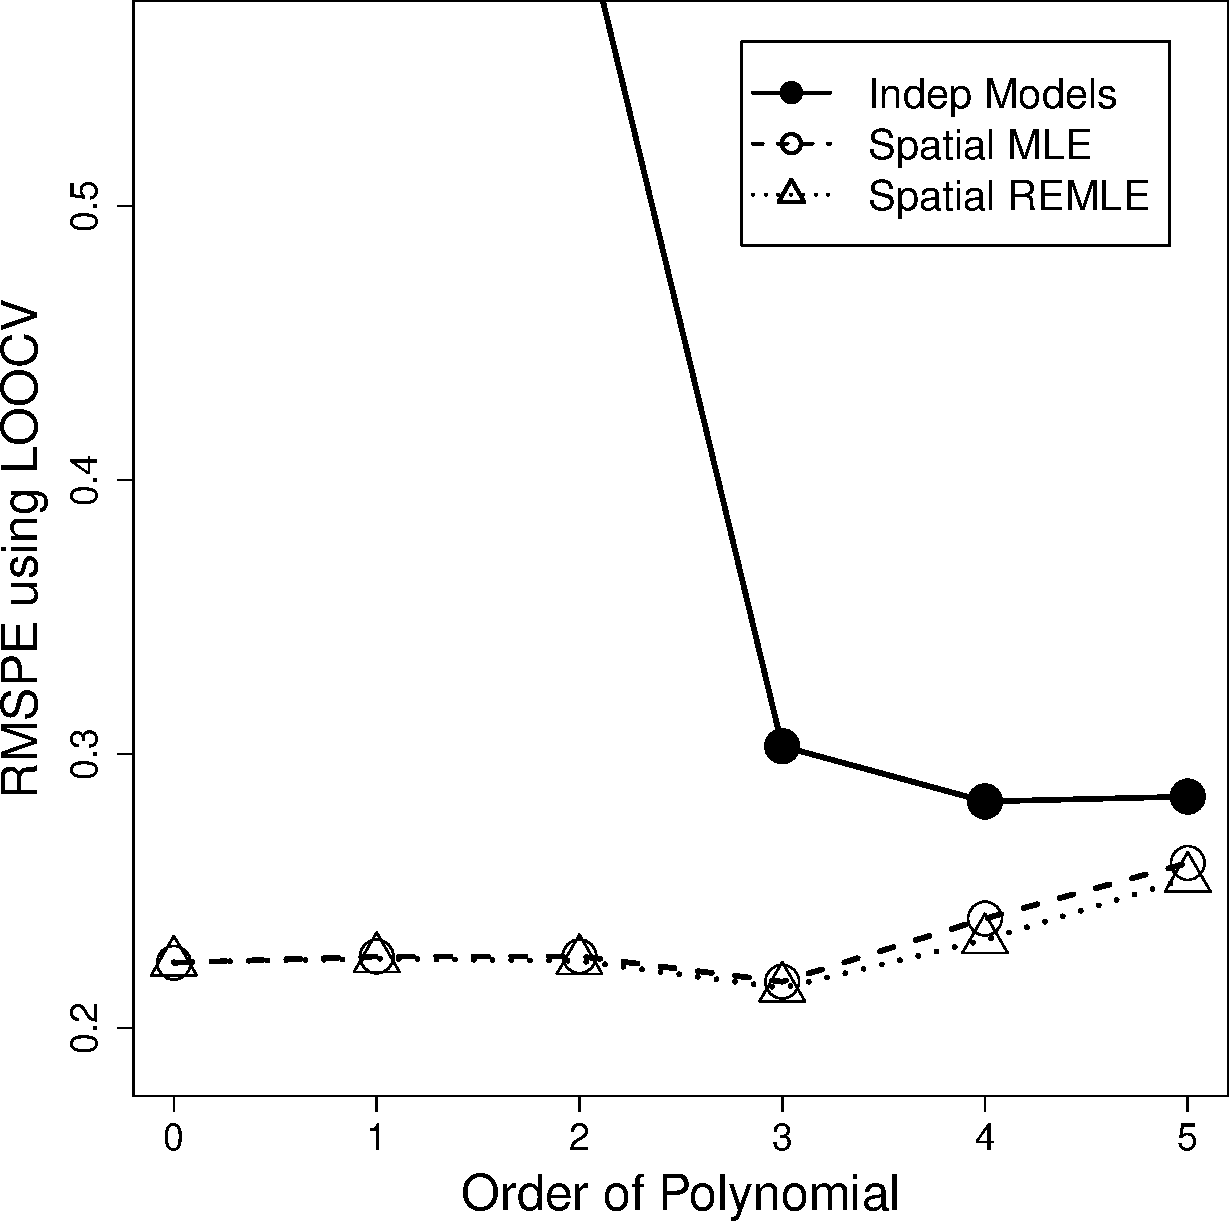
\includegraphics[width=.5\linewidth]{SO4_LOOCV}
  \end{center}
  \caption{LOOCV for polynomial models on the spatial coordinates, for independent error models (solid line and circle) and spatial models with ML estimation (dashed line and open circles) and REML estimation (dotted line with open triangles). \label{Fig:SO4_LOOCV}}
\end{figure}

%%%%%%%%%%%%%%%%%%%%%%%%%%%%%%%%%%%%%%%%%%%%%%%%%%%%%%%%%%%%%%%%%%%%%%%%%%%%%%%%%%
%%%%%%%%%%%%%%%%%%%%%%%%%%%%%%%%%%%%%%%%%%%%%%%%%%%%%%%%%%%%%%%%%%%%%%%%%%%%%%%%%%
%                BIBLIOGRAPHY
%%%%%%%%%%%%%%%%%%%%%%%%%%%%%%%%%%%%%%%%%%%%%%%%%%%%%%%%%%%%%%%%%%%%%%%%%%%%%%%%%%
%%%%%%%%%%%%%%%%%%%%%%%%%%%%%%%%%%%%%%%%%%%%%%%%%%%%%%%%%%%%%%%%%%%%%%%%%%%%%%%%%%

%\bibliographystyle{consbiol}
\bibliographystyle{/media/jay/Hitachi2GB/shTex/asa}
\bibliography{/media/jay/Hitachi2GB/shTex/StatBibTex.bib}
%\bibliographystyle{/home/jay/Data/shTex/shTex/asa}
%\bibliography{/home/jay/Data/shTex/shTex/StatBibTex.bib}




\end{document}

